\documentclass[utf8, aspectratio=169]{beamer}
\mode<presentation>
\usetheme{metropolis}
\metroset{block=fill}
\usepackage{pgf}
\usepackage{tikz}
\usetikzlibrary{shapes, arrows.meta, positioning, calc, graphs, fit, backgrounds}
\usepackage[T1]{fontenc}
\usepackage[utf8]{inputenc}
\usepackage[portuguese]{babel}
\usepackage{multicol}
\usepackage{graphicx}
\usepackage{mathtools}
\mathtoolsset{mathic}
\usepackage{listings}
\usepackage[style=authoryear,backend=biber]{biblatex}
\addbibresource{main.bib}

\definecolor{cdpgray}{HTML}{E4DDD9}
\definecolor{cdplightgreen}{HTML}{ABCCBD}
\definecolor{cdpdarkgreen}{HTML}{7DBEB8}
\definecolor{cdpblack}{HTML}{19171A}
\definecolor{cdpred}{HTML}{E33F21}

\setbeamercolor{normal text}{fg=cdpblack, bg=cdpgray}
\setbeamercolor{alerted text}{fg=cdpred}
\setbeamercolor{example text}{fg=cdpdarkgreen}

\setbeamercolor{palette primary}{bg=cdpblack, fg=cdpgray}
\setbeamercolor{palette secondary}{bg=cdpdarkgreen, fg=cdpblack}
\setbeamercolor{palette tertiary}{bg=cdpblack, fg=cdpgray}
\setbeamercolor{palette quaternary}{bg=cdpblack, fg=cdpgray}

\setbeamercolor{structure}{fg=cdpblack}
\setbeamercolor{frametitle}{bg=cdpblack, fg=cdpgray}

\setbeamercolor{block title}{bg=cdpblack, fg=cdpgray}
\setbeamercolor{block body}{bg=white, fg=cdpblack}
\setbeamercolor{block title alerted}{bg=cdpred, fg=white}
\setbeamercolor{block body alerted}{bg=white, fg=cdpblack}
\setbeamercolor{block title example}{bg=cdpdarkgreen, fg=cdpblack}
\setbeamercolor{block body example}{bg=white, fg=cdpblack}

\addtobeamertemplate{frametitle}{}{%
  \begin{tikzpicture}[remember picture,overlay]
    \node[anchor=north east, yshift=0.0cm, xshift=-0.2cm] at (current page.north east) {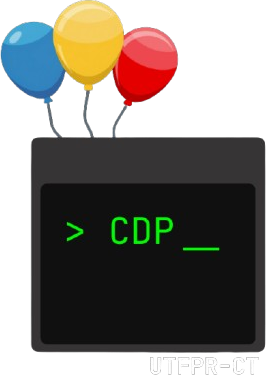
\includegraphics[height=0.7cm]{images/logo_cdp-branco.png}};
  \end{tikzpicture}
}

\definecolor{keywordcolor}{rgb}{0.0,0.0,0.7}
\definecolor{commentcolor}{rgb}{0.0,0.5,0.0}
\definecolor{stringcolor}{rgb}{0.58,0,0.82}
\definecolor{typecolor}{rgb}{0.2,0.2,0.6}
\definecolor{idcolor}{rgb}{0.55,0.0,0.1}


\lstdefinelanguage{C++Custom}{
    language=C++,
    morekeywords={[2]int, float, double, bool, char, void, string},
    morekeywords={[3]std, cout, cin, endl},
    sensitive=true
}

\lstdefinestyle{cpp}{
    language=C++Custom,
    basicstyle=\ttfamily\scriptsize,
    keywordstyle=\color{keywordcolor}\bfseries,
    commentstyle=\color{commentcolor}\itshape,
    stringstyle=\color{stringcolor},
    identifierstyle=\color{idcolor},
    numbers=left,
    numberstyle=\tiny,
    stepnumber=1,
    numbersep=5pt,
    showstringspaces=false,
    tabsize=4,
    breaklines=true,
    captionpos=b,
    xleftmargin=10pt
}

\lstset{style=cpp}


\title{Template de Apresentação}
\subtitle{Clube de Programação -- UTFPR-CT}
\author{Nome do Apresentador}
\institute{Universidade Tecnológica Federal do Paraná, Campus Curitiba}
\date{\today}

% Adding the logo to the title page
\titlegraphic{\vspace{4.5cm}\flushright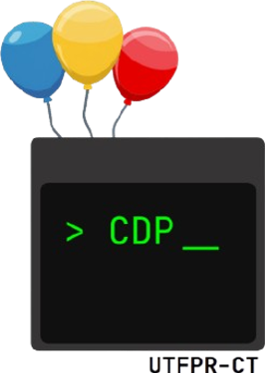
\includegraphics[width=2.5cm]{images/logo_cdp-preto.png}}

\begin{document}

\begin{frame}[plain,noframenumbering]
  \titlepage
\end{frame}

\begin{frame}{Sumário}
  \setbeamertemplate{section in toc}[sections numbered]
  \tableofcontents[hideallsubsections]
\end{frame}

\section{Introdução}

\begin{frame}{Listas e Textos Básicos}
  \begin{itemize}
    \item Este é um template base para o \alert{Clube de Programação}.
    \item Ele foi desenvolvido para aulas do básico ao nível avançado \parencite{halim2013competitive}.
    \item Você pode utilizar \alert{texto em destaque} ou criar listas enumeradas:
  \end{itemize}
  
  \begin{enumerate}
    \item Primeiro passo.
    \item Segundo passo com matemática inline: $O(N \log N)$.
    \item Terceiro passo.
  \end{enumerate}
\end{frame}

\begin{frame}{Documentação e Ferramentas}
  Este template foi construído utilizando as seguintes ferramentas:
  \vspace{0.5cm}
  \begin{itemize}
    \item \textbf{Beamer}: Classe LaTeX para criação de apresentações. \\
          \url{https://ctan.org/pkg/beamer}
    \vspace{0.3cm}
    \item \textbf{Tema Metropolis}: O design moderno e minimalista utilizado. \\
          \url{https://github.com/matze/mtheme}
    \vspace{0.3cm}
    \item \textbf{TikZ}: Pacote para criação de gráficos e diagramas vetoriais. \\
          \url{https://tikz.dev/}
  \end{itemize}
\end{frame}

\begin{frame}[fragile]{Como usar este template}
  \textbf{No Linux (Localmente)}
  \begin{itemize}
    \item Instale a distribuição completa do TeX Live (em distribuições baseadas em Debian/Ubuntu):
    \begin{lstlisting}[language=bash, numbers=none, xleftmargin=0em, framexleftmargin=0em]
sudo apt install texlive-full
    \end{lstlisting}
    \item Para compilar o projeto, basta rodar o comando \texttt{make} no terminal. O \texttt{Makefile} já cuida de limpar arquivos auxiliares e compilar a bibliografia corretamente.
  \end{itemize}

  \vspace{0.3cm}
  \textbf{No Overleaf (Nuvem)}
  \begin{itemize}
    \item Crie um \textbf{Novo Projeto Vazio}.
    \item Faça o upload de todos os arquivos (\texttt{main.tex}, \texttt{main.bib} e a pasta \texttt{images/}).
    \item O Overleaf vai detectar o \texttt{main.tex} automaticamente e compilar o PDF.
  \end{itemize}
\end{frame}

\section{Estruturas de Dados Visuais}

\begin{frame}{Grafos (Nós e Arestas)}
  \begin{center}
    \begin{tikzpicture}[
      node distance=1.5cm and 2.5cm,
      v/.style={circle, draw=cdpblack, fill=cdplightgreen, minimum size=7mm, thick},
      e/.style={thick, cdpblack},
      ered/.style={thick, cdpred},
      egreen/.style={thick, cdpdarkgreen}
    ]
      \node[v] (1) {1};
      \node[v] (2) [above right=of 1] {2};
      \node[v] (3) [below right=of 1] {3};
      \node[v] (4) [below right=of 2] {4};
      \node[v, fill=white] (5) [right=of 4] {5};

      \draw[e] (1) -- node[above left, font=\small] {2} (2);
      \draw[ered] (1) -- node[below left, font=\small] {5} (3);
      \draw[egreen, ->, >=Stealth] (2) -- node[above right, font=\small] {1} (4);
      \draw[e] (3) -- node[below right, font=\small] {3} (4);
      \draw[e, dashed] (2) -- node[right, font=\small] {4} (3);
      \draw[e, <->, >=Stealth] (4) -- node[above, font=\small] {8} (5);
    \end{tikzpicture}
  \end{center}
\end{frame}

\begin{frame}{Vetores (Arrays 1D)}
  \begin{center}
    \begin{tikzpicture}[
      cell/.style={rectangle, draw=cdpblack, thick, minimum width=1.2cm, minimum height=1.2cm, anchor=center},
      idx/.style={above, font=\scriptsize, text=cdpdarkgreen}
    ]
      \node[cell] (A0) {10};
      \node[cell, right=-\pgflinewidth of A0] (A1) {25};
      \node[cell, right=-\pgflinewidth of A1] (A2) {8};
      \node[cell, fill=cdplightgreen, right=-\pgflinewidth of A2] (A3) {42};
      \node[cell, right=-\pgflinewidth of A3] (A4) {7};
      \node[cell, right=-\pgflinewidth of A4] (A5) {15};
      \node[cell, right=-\pgflinewidth of A5] (A6) {3};
      
      \foreach \i in {0,...,6} {
        \node[idx] at (A\i.north) {\i};
      }
      
      \draw[->, thick, cdpred, >=Stealth] (A3.south) ++(0,-0.6) -- node[below=6pt] {Máximo} (A3.south);
      \draw[->, thick, cdpblack, >=Stealth] (A1.south) ++(0,-0.6) -- node[below=6pt] {$i$} (A1.south);
    \end{tikzpicture}
  \end{center}
\end{frame}

\begin{frame}{Matrizes (Arrays 2D)}
  \begin{center}
    \begin{tikzpicture}[
      cell/.style={rectangle, draw=cdpblack, thick, minimum width=1.2cm, minimum height=1.2cm, anchor=center}
    ]
      \node[cell] (M00) {0};
      \node[cell, right=-\pgflinewidth of M00] (M01) {1};
      \node[cell, right=-\pgflinewidth of M01] (M02) {1};
      \node[cell, right=-\pgflinewidth of M02] (M03) {0};
      
      \node[cell, below=-\pgflinewidth of M00] (M10) {1};
      \node[cell, fill=cdpdarkgreen, text=white, right=-\pgflinewidth of M10] (M11) {0};
      \node[cell, right=-\pgflinewidth of M11] (M12) {0};
      \node[cell, right=-\pgflinewidth of M12] (M13) {1};
      
      \node[cell, below=-\pgflinewidth of M10] (M20) {1};
      \node[cell, fill=cdpred, text=white, right=-\pgflinewidth of M20] (M21) {1};
      \node[cell, right=-\pgflinewidth of M21] (M22) {0};
      \node[cell, right=-\pgflinewidth of M22] (M23) {0};
      
      \node[cell, below=-\pgflinewidth of M20] (M30) {0};
      \node[cell, right=-\pgflinewidth of M30] (M31) {1};
      \node[cell, right=-\pgflinewidth of M31] (M32) {0};
      \node[cell, right=-\pgflinewidth of M32] (M33) {0};
      
      % Row indices
      \foreach \i in {0,...,3} {
        \node[left=0.2cm, font=\scriptsize, text=cdpdarkgreen] at (M\i0.west) {\i};
      }
      % Col indices
      \foreach \i in {0,...,3} {
        \node[above=0.2cm, font=\scriptsize, text=cdpdarkgreen] at (M0\i.north) {\i};
      }
    \end{tikzpicture}
  \end{center}
\end{frame}

\section{Algoritmos e Matemática}

\begin{frame}{Relações de Recorrência}
  \begin{block}{Sequência de Fibonacci}
    A sequência de Fibonacci é definida pela seguinte relação de recorrência:
    \begin{equation*}
      F(n) = 
      \begin{cases}
        0 & \text{se } n = 0 \\
        1 & \text{se } n = 1 \\
        F(n-1) + F(n-2) & \text{se } n > 1
      \end{cases}
    \end{equation*}
  \end{block}
  \begin{exampleblock}{Exemplo de Computação}
    Avaliando a função:
    $$F(4) = F(3) + F(2) = (F(2) + F(1)) + (F(1) + F(0)) = \dots = 3$$
  \end{exampleblock}
\end{frame}

\begin{frame}{Ilustrando Processos Passo a Passo}
  \begin{center}
    \Large Exemplo: Bubble Sort
    \vspace{1cm}

    \begin{tikzpicture}[
      cell/.style={rectangle, draw=cdpblack, thick, minimum width=1.2cm, minimum height=1.2cm, anchor=center}
    ]
      \node[cell] (A1) {5};
      \node[cell, right=-\pgflinewidth of A1] (A2) {2};
      \node[cell, right=-\pgflinewidth of A2] (A3) {9};
      \node[cell, right=-\pgflinewidth of A3] (A4) {1};
      \node[cell, right=-\pgflinewidth of A4] (A5) {8};
      
      \uncover<2-3>{
        \draw[<->, thick, cdpred, >=Stealth] (A1.south) ++(0,0) to[bend right] (A2.south);
        \node[below=0.8cm of A1, xshift=0.6cm, text=cdpred] {Swap!};
      }
      
      \uncover<3->{
        \node[cell, fill=cdplightgreen] at (A1) {2};
        \node[cell, fill=cdplightgreen] at (A2) {5};
      }
      
      \uncover<4->{
        \draw[<->, thick, cdpred, >=Stealth] (A3.south) ++(0,0) to[bend right] (A4.south);
        \node[below=0.8cm of A3, xshift=0.6cm, text=cdpred] {Swap!};
      }

      \uncover<5->{
        \node[cell, fill=cdplightgreen] at (A3) {1};
        \node[cell, fill=cdplightgreen] at (A4) {9};
      }

      \uncover<6->{
        \node[cell, below=2cm of A1] (B1) {2};
        \node[cell, right=-\pgflinewidth of B1] (B2) {5};
        \node[cell, right=-\pgflinewidth of B2] (B3) {1};
        \node[cell, right=-\pgflinewidth of B3] (B4) {8};
        \node[cell, fill=cdpblack, text=white, right=-\pgflinewidth of B4] (B5) {9};
        
        \node[left=0.5cm of B1] {Estado Final:};
      }

    \end{tikzpicture}
  \end{center}
\end{frame}

\begin{frame}{Setas e Fluxogramas}
  \begin{center}
    \begin{tikzpicture}[
      box/.style={rectangle, draw=cdpblack, fill=white, rounded corners, thick, minimum width=2.5cm, minimum height=1cm, align=center},
      arr/.style={-{Stealth[scale=1.2]}, thick, cdpblack}
    ]
      \node[box] (A) {Código Fonte \\ \texttt{main.cpp}};
      \node[box, right=1cm of A] (B) {Compilador \\ \texttt{g++}};
      \node[box, right=1cm of B] (C) {Executável \\ \texttt{a.out}};
      
      \node[box, fill=cdplightgreen, above=1.2cm of C] (D) {Entrada \\ (Casos de Teste)};
      \node[box, fill=cdpdarkgreen, below=1.2cm of C] (E) {Saída \\ (Resultados)};
      
      \draw[arr] (A) -- (B);
      \draw[arr] (B) -- (C);
      \draw[arr] (D) -- (C);
      \draw[arr] (C) -- (E);
    \end{tikzpicture}
  \end{center}
\end{frame}

\begin{frame}{Geometria: Convex Hull (Monotonic Chain)}
  \begin{center}
    \begin{tikzpicture}[scale=0.85, transform shape]
      % Grid
      \draw[step=1cm, cdpgray, very thin, dashed] (-0.5,-0.5) grid (6.5, 4.5);
      
      % Eixos
      \draw[->, thick, cdpblack] (-0.5,0) -- (6.5,0) node[right] {$x$};
      \draw[->, thick, cdpblack] (0,-0.5) -- (0,4.5) node[above] {$y$};

      % Coordenadas
      \coordinate (P0) at (0,2);
      \coordinate (P1) at (1,0);
      \coordinate (P2) at (2,2);
      \coordinate (P3) at (3,1);
      \coordinate (P4) at (4,4);
      \coordinate (P5) at (5,1);
      \coordinate (P6) at (6,3);

      % Lower Hull
      \uncover<2->{
        \draw[thick, cdpred, ->, >=Stealth] (P0) -- (P1);
        \draw[thick, cdpred, ->, >=Stealth] (P1) -- (P5);
        \draw[thick, cdpred, ->, >=Stealth] (P5) -- (P6);
        \node[cdpred, below right] at (P5) {Lower Hull};
      }

      % Upper Hull
      \uncover<3->{
        \draw[thick, cdpdarkgreen, ->, >=Stealth] (P6) -- (P4);
        \draw[thick, cdpdarkgreen, ->, >=Stealth] (P4) -- (P0);
        \node[cdpdarkgreen, above right] at (P4) {Upper Hull};
      }

      % Pontos
      \foreach \i in {0,...,6} {
        \node[circle, fill=cdpblack, inner sep=1.5pt] (N\i) at (P\i) {};
        \node[above=2pt, font=\scriptsize] at (N\i) {$P_\i$};
      }
      
      % Pontos ignorados
      \uncover<4->{
        \node[circle, fill=gray, inner sep=1.5pt] at (P2) {};
        \node[circle, fill=gray, inner sep=1.5pt] at (P3) {};
      }
    \end{tikzpicture}
  \end{center}
  
  \vspace{-0.5cm}
  \begin{itemize}
    \item<1-> \textbf{Passo 1:} Ordenar pontos por coordenada $x$ (e $y$ em caso de empate).
    \item<2-> \textbf{Passo 2:} Construir o {\color{cdpred}\textbf{Lower Hull}} (remover curvas à direita).
    \item<3-> \textbf{Passo 3:} Construir o {\color{cdpdarkgreen}\textbf{Upper Hull}} (remover curvas à direita).
    \item<4-> Pontos internos ($P_2, P_3$) são descartados pelo produto vetorial.
  \end{itemize}
\end{frame}

\section{Imagens e Código}

\begin{frame}{Mostrando Imagens}
  As imagens podem ser incluídas facilmente utilizando o pacote \texttt{graphicx}. O template pode misturar imagens e blocos.

  \begin{figure}
    \centering
    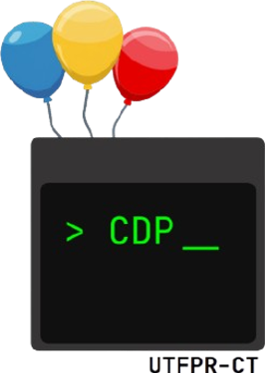
\includegraphics[height=3.5cm]{images/logo_cdp-preto.png}
    \caption{Logo oficial do CDP}
  \end{figure}
\end{frame}

\begin{frame}[fragile]{Visualização de Código Fonte}
  Útil para mostrar implementações de algoritmos durante os encontros do clube.
  \vspace{0.5cm}
  
  \begin{lstlisting}
#include <bits/stdc++.h>
using namespace std;

// Exemplo de busca binaria
int binary_search(const vector<int>& arr, int target) {
    int l = 0, r = arr.size() - 1;
    while (l <= r) {
        int mid = l + (r - l) / 2;
        if (arr[mid] == target) return mid;
        if (arr[mid] < target) l = mid + 1;
        else r = mid - 1;
    }
    return -1;
}
  \end{lstlisting}
\end{frame}

\begin{frame}[plain,noframenumbering]
  \begin{center}
    % \vspace{2cm}
    {\Huge \textbf{Dúvidas?}}
    
    % \vspace{1cm}
    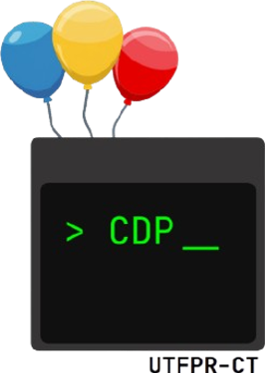
\includegraphics[width=4cm]{images/logo_cdp-preto.png}
    
    \vspace{0.5cm}
    {\large Clube de Programação -- UTFPR-CT}
  \end{center}
\end{frame}

\begin{frame}[allowframebreaks]{Referências}
  \printbibliography
\end{frame}

\end{document}
